\documentclass[a4wide, 11pt]{article}
\usepackage{a4, fullpage}
\usepackage[pdftex]{graphicx} \DeclareGraphicsRule{*}{mps}{*}{}
\usepackage{enumerate}
\usepackage{hyperref}
\setlength{\parskip}{0.3cm}
\setlength{\parindent}{0cm}

% This is the preamble section where you can include extra packages etc.

\begin{document}

\title{WebApps Group Project: Project Report}

\author{Duc Ngo \and Roozbeh Zareian \and Ningyuan Lu}

\date{\today}         % inserts today's date

\maketitle            % generates the title from the data above

\section{Introduction}

For our WebApps Project, we decided to write a web-based game. Our primary aim is to get our website to work properly, ie a working register and log-in form. 

We use database to allow players to have an account in our website and login to play , we give every new play a unique identification and it will keep tracking player’s activities including the resources he had already and how big the map he has explored . All player’s information will be store in the database . We also use database to deal with some global events ,such as leaving messages in a certain place and other players is able to write or edit that.

For the game, we aim to create a sandbox-ish kind of game where players can gather resources, construct buildings and most importantly, interact with other players who are playing at the same time.

\section{Project Management}
\subsection{Group Structure}

We have 3 people in our group. None of us has any experience in game programming or web programming, so we decided to split our work somewhat based on personal preference. 

Yan designs database and writing PHP files in the server end . 
First thing is to create the registration and login system with validate name and password checking properties .Gamers should firstly create their account in our website and then he can login with an unique player ID which been given by the server to play our games .
Second thing is to make a communication from between game and database through the server . Everything in the game which need to be stored in the database he deal with them .

Duc designs the core of the game, edit the map and writes the game logic code and Roozbeh designs the website and the game’s graphics.

\subsection{Project Management}

\textbf{GAME DESIGN (Duc)}

I chose to use JavaScript because of its good support for most browsers. It also has a wide variety of libraries and tools that I can use to speed up my progress, especially when I
have no background on JavaScript and a very limited knowledge on HTML.

After some research, I decided to use a game engine to help me on designing and coding the game. It’s also a good opportunity to learn JavaScript and game programming.

There are many game engines on the net but many of them are not free and/or complicate to use, requiring backgrounds on JavaScript. So I decided to use Crafty, a free and open source JavaScript game library.

\url{http://craftyjs.com/}

or even

\url{https://github.com/craftyjs/Crafty}

This engine is, in my opinion, good for Web Game programming. It’s really small (300kb file) and simple to install, I only need to include 1 .js file to my library. It also support either DOM or Canvas rendering, flexibility is always good. Components and entities management is also simple and makes sense, which is better than using JavaScript’s prototypes model. More importantly it has support for different community modules so I can choose whatever I need. 

However even though the Crafty community is quite active, it’s still hard to find a thorough tutorial on different topics that I have to cover in order to transform the game from an idea into a real thing.

After grasping the basics of game programming, I stumbled into the problem of map creation. In my initial design, our game includes a random map generator. That idea quickly came to an end after I realise how much work needs to be put into that (I’ll work on it in Summer!). Still, map creation is tedious and hard to do without a tool. For the purpose of demonstration, I figured I need to create a demo map for our game, especially when our game is tile-based.

I decided to use Tiled Map Editor, another free and powerful tool to help me in this quest.

\url{http://www.mapeditor.org/}

or

\url{https://github.com/bjorn/tiled}

This map editor can help me create layers and add properties to tiles. Grabbing images from sprites is also easy with the help of it.

\includegraphics[width=\linewidth]{Tiled}

The only problem I have with this is the lack of tutorials. I enjoy learning to use these new tools and languages, but our time is also limited.

I used a free and open source component to help me import the map from Tiled Map Editor to JavaScript.

\url{https://github.com/Kibo/TiledMapBuilder}


\textbf{DATABASE COMMUNICATION (YAN)}

\textbf{Language and software I choose :}

\textbf{Apache HTTP Server }

I use Apache HTTP Server for make the localhost. (\url{http://httpd.apache.org/})

Reason:

Apache HTTP Server is world’s largest free and open source HTTP server , compare to Microsoft IIS , the most benefit for me is Apache is free and it’s cross platform since I work with Mac OS , Microsoft only work with windows platform and it’s been bundled with Windows NT.

And also, Apache is stable and easy to deploy,it’s mature since been developed from 1995.  

\textbf{Javascript and AJAX}

We use Javascript in almost everywhere in the client design ,and it’s been discussed by Duc in previous session. 

AJAX is a good way to communicate between javascript and PHP, faster and really easy to implement.by using AJAX I do not need to connect the webpage to the server every time, and it’s easy to updating datas,AJAX selecting contents from web which need to be update and then send them to server to deal with them . 

\textbf{Hypertext Preprocessor (PHP)}

I decided to choose Ruby on rails first , but PHP+MYSQL+APACHE is very popular, and PHP is easy to learn and convenience to construct a simple website , so I switch to PHP at last . PHP is a very popular language and lot’s website using that. But I know Ruby on Rails is modern and cool, so after I learn some basic stuff in PHP I will switch to ruby in future.

\textbf{PostgreSQL}

\url{http://www.postgresql.org/}

I finally choose postgreSQL instead of MySQL because MySQL is too wildly use , and since PostgreSQL is ‘world’s most advance open source database’ , it’s stable and advance , I think it’s worth to learn how to use it.

\textbf{Eclipse IDE for Java EE developers with plugins}

\url{http://www.eclipse.org/downloads/packages/eclipse-ide-java-ee-developers/junosr2}

This famouse IDE have almost any plugins you want , by using IDE I can minimize the bugs when I trying to learn a new language . It also gives you a good vision of your file location and properties inside your code , which makes me easy and fast to write some prototype code in current stage . 

\textbf{Google Chrome and PHP console plugin}

I’ve been use Google Chrome for couple of years it’s still be my favourite web browser to use .

By pressing command+option+J to bring out the console it’s really easy for me to inspect bugs and element’s inside the code.

I also install a plugin called \textbf{PHP console}

\url{https://chrome.google.com/webstore/detail/php-console/nfhmhhlpfleoednkpnnnkolmclajemef}

By implementing a debug library in my PHP file it will display PHP bugs in Google Chrome’s console, really easy to use.

\subsection{Version Control}

We used github.com to keep track of our code. Before this Project, we also worked together on Pintos and also used github, so using git is quite natural to us. It’s also a good way to keep our project backed up.

\includegraphics[width=\linewidth]{git1}

\includegraphics[width=\linewidth]{git2}

We also set up a googledocs to keep track of what we’ve done, what we need to do and progress on different tasks.

\section{Program Description}
\subsection{Game}

As stated in the milestone report, our game is a web-based game that is influenced by \textit{Dwarf Fortress, Dark Souls} and \textit{Don’t Starve}.

A player will play the role of a Wizard, trapped on an Island without any apparent means to escape. Players can choose a profession, be it Carpenter, Mason or Miner, and a spell school: Fire, Lightning or Ice . Each profession can only gather the related resources and build related structures. For example: a Carpenter can only chop down trees and create wooden houses, a Miner can only mine minerals and create weapons. etc.

There will be also a special resource called \textit{Soul}, which can only be acquired by killing bosses in the game or fighting other players.

In order to win the game, players are required to gather all types of resources, including Souls, so naturally there will be tradings and fighting between players of different professions.

We use a system of ‘summoning’ to handle this. There can be more than 1 player presenting in the game server but they will not see each other, each will be in their own ‘parallel’ island. However, as they are powerful wizards, they can send messages through other universes. Players can put down a message anywhere they can go to. Other players playing at the same time can see that ‘message’ object and can read it, and even add more to it. This system can help players communicate, to warn others about danger ahead, to ask for trading, or even to trick others.

There is also a ‘summoning’ sign that players can put down. Similarly to the ‘messages’, these signs can be seen by other players, and when someone decided to activate it (let’s call him the ‘host’), the person who put it down can be summoned into the ‘host’s world. There, they can start trading or fighting the ‘host’. Only the ‘summoned’ can start the fighting, to avoid people building traps then summon people just to kill them.

We also want to implement a system of hidden events. There can be random events and static events. Static events will be triggered when the player step into a particular tile (people can warn each other about these events via putting down messages nearby, or not, just to be evil). Random events can happen anywhere.

About design patterns, being unfamiliar with game programming, I followed a few different tutorials on how to organise my files and resources. It is basically a MVC pattern, with the map loading and drawing, game logic and events, player controller separated.

\subsection{Database and Server}

I use MVC model to connect to our database , View will be front end design including HTML page and Javascript inside it , Controller will be PHP files which been stored in the server , Model is the actual database and queries . 

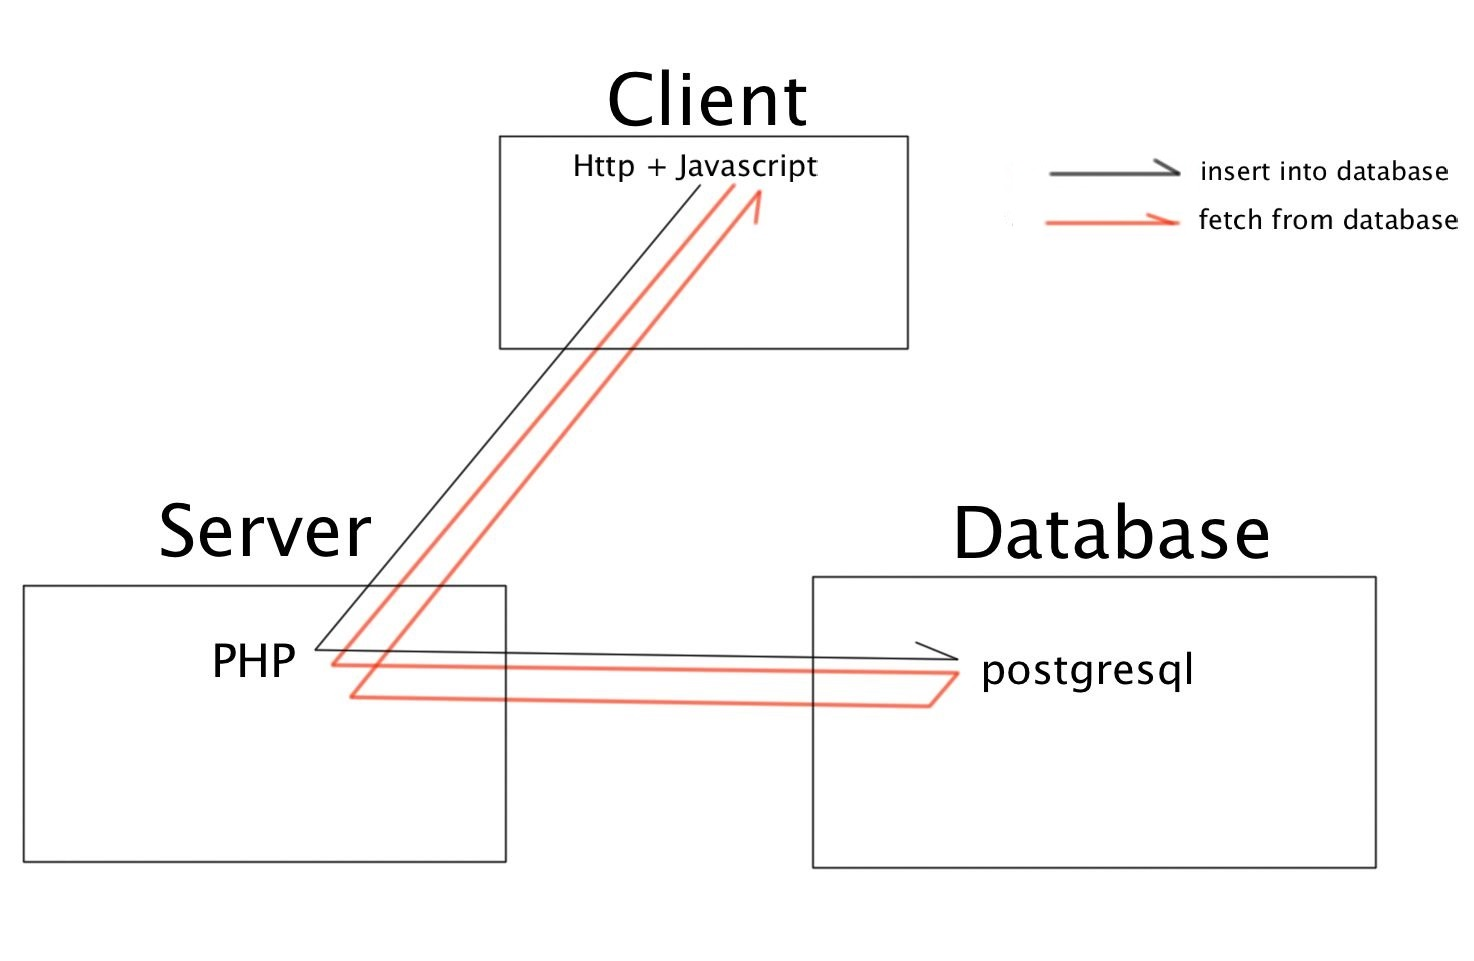
\includegraphics[width=\linewidth]{comm}


The most important reason I use MVC model is for security reason . Because if we use javascript directly connect to the database without using PHP then the gamer is easy to manipulate the database directly by changing the javascript code . And also , by using MVC model it’s easy to control and tracking whole game data when the game is becoming bigger .

And also , I created three tables inside the database which deal with different functions of the game:

\textit{\textbf{register\_table for Registration and Login}}

First table is called \textit{register\_table}, which contain three columns, ID, username,password . When a player successfully created their account by typing valid username and password, database will automatically give them an unique game ID.

\textit{\textbf{player\_table for Storing Player’s Status and Information}}

ID will be the primary key to another table called \textit{player\_table} ,it contains n columns which stored all player’s personal information in a single row. ID, Wood ,Soul,and more after we keep developing our games .

\textit{\textbf{message\_table for Global Message }}

There will be a third table which called \textit{message\_table} , this table is used for leaving player global message . There is no column called ID because the message will displayed anonymously. There will be three columns inside this table ,X,Y,Message. X,Y is the location of this message. This table will be keep tracking during the gaming, if someone leave messages and this message will display immediately on others’ map. Once the message been placed,there is no chance to delete it , the only thing player can do is add more text in it . I will deal with this function in the server.

\textit{\textbf{Map Resources Tracking Property}}

Since every player will have an unique map ,which means the resources will not be shared , I solve this by creating new map which specific to this play in the server . 

Once a player register on our website and get the system generated ID, automatically a map file called map\_[id].json will be copied from map.json automatically (map.json is the default map we created) as his personal map. 

When player login to our game his personal map will be fetched out as his map .When he interacting with the game resources been placed on the map , it will only modificate his own mapfile.Next time he login , every interaction he is done before will still be there.

\section{Acknowledgement}

For the sprites and small images, most of them are taken from Google Images Search. I made sure to check for the poster’s remark about this. In some cases, we sent an email to the author to ask for their permission to use them.

Crafty Game engine: \url{https://github.com/craftyjs/Crafty}

Tiled Map Editor: \url{https://github.com/bjorn/tiled}

Kibo’s TiledMapBuilder: \url{https://github.com/Kibo/TiledMapBuilder}

\section{Conclusion}

For now, our aim to create a fully playable game has failed. We only have enough time to create a demo map, where a player can start gathering some resources, building some of the buildings and we only have the messaging system, not summoning.

What we still have to work on:

\begin{itemize}
\item
Profession System

\item
Items and Spells System

\item
Combat System

\item
Summoning System

\item
A fully implemented building and upgrade tree

\item
A better UI

\item
A more optimised loading time and general performance

\item
General game balance
\end{itemize}

\subsection{Good}

The Project was a fun experience. We really enjoy learning JavaScript. Researching about game programming is also interesting. We think if we have more time, we can definitely make this a good game. However as we gain more experience in the field, we may choose other game engines, tools and libraries. For this project, we pretty much chose what other people think is good, without deep knowledge about other tools.

\subsection{Bad}

We haven’t match our initial aim. Our JavaScript code is still very messy and not optimal, so it’s still hard to expand what we have right now.

\subsection{What we've learned}

For now we have gained a good amount of web game programming experience. During our work, we were able to create some small games just to practice and for fun. (Duc) I actually want to finish the game as a side project during Summer.


\end{document}

